\documentclass[11pt,a4paper]{report}
% dasselbe Template wie Thesis mit nur leichten Anpassungen
% Nehmen Sie das Thesis-Template für die Thesis!
% Lesen Sie Hinweise zum Umgang mit LaTeX und zum Schreiben
% von Berichten im Thesis-Template nach
% => Moodle => PraxissemesterThesis => LaTeXThesis.zip
%    https://moodle.hs-mannheim.de/course/view.php?id=2500


% Für doppelseitigen Ausdruck (nur bei > 60 Seiten sinnvoll)
% \usepackage{ifthen}
% \setboolean{@twoside}{true}
% \setboolean{@openright}{true} 

% pakete
\usepackage{ifthen}

% Deutsch
\usepackage[german]{babel} % deutsch und deutsche Rechtschreibung
\usepackage[backend=biber, style=numeric, sorting=none]{biblatex} % Literaturverzeichnis (sortiert nach Reihenfolge des Auftretens)
\addbibresource{praksem.bib}
\usepackage[utf8]{inputenc} % Unicode Text
\usepackage[T1]{fontenc} % Umlaute und deutsches Trennen
\usepackage{textcomp} % Euro
% statt immer Ab\-schluss\-ar\-beit zu schreiben
% einfach hier sammeln mit -. 
\hyphenation{Ab-schluss-ar-beit}
% Vorsicht bei Umlauten und Bindestrichen
\hyphenation{Ver-st\"ar-ker-aus-gang}
 % eigene Hyphenations, die für das Dokument gelten
\usepackage{amssymb} % Symbole
\usepackage{emptypage} % Wirklich leer bei leeren Seiten

%% Fonts, je ein kompletter Satz an Optionen

% Times New Roman, gewohnter Font, ok tt und serifenlos
%\usepackage{mathptmx} 
%\usepackage[scaled=.95]{helvet}
%\usepackage{courier}

% Palatino mit guten Fonts für tt und serifenlos
\usepackage{mathpazo} % Palatino, mal was anderes
\usepackage[scaled=.95]{helvet}
\usepackage{courier}

% New Century Schoolbook sieht auch nett aus (macht auch tt und serifenlos)
%\usepackage{newcent}

% Oder default serifenlos mit Helvetica 
% ich kann es nicht mehr sehen ...
%\renewcommand{\familydefault}{\sfdefault}

% ein bisschen eine bessere Verteilung der Buchstaben...
\usepackage{microtype}

% Bilder und Listings
\usepackage{graphicx} % wir wollen Bilder einfügen
\usepackage{subfig} % Teilbilder
\usepackage{wrapfig} % vielleicht doch besser vermeiden
\usepackage{listings} % schöne Quellcode-Listings
% ein paar Einstellungen für akzeptable Listings
\lstset{basicstyle=\ttfamily, columns=[l]flexible, mathescape=true, showstringspaces=false, numbers=left, numberstyle=\tiny}
\lstset{language=python} % und nur schöne Programmiersprachen ;-)
% und eine eigene Umgebung für Listings
\usepackage{float}
\newfloat{listing}{htbp}{scl}[chapter]
\floatname{listing}{Listing}

% Seitenlayout
\newcommand{\seitenseitenabstand}{22mm} % 30mm
\usepackage[paper=a4paper,left=\seitenseitenabstand,right=\seitenseitenabstand,height=23cm]{geometry}
\usepackage{setspace}
% \linespread{1.15}
\linespread{1.1}
\setlength{\parskip}{0.5em}
\setlength{\parindent}{0em} % im Deutschen Einrückung nicht üblich, leider

% Seitenmarkierungen 
\newcommand{\phv}{\fontfamily{phv}\fontseries{m}\fontsize{9}{11}\selectfont}
\usepackage{fancyhdr} % Schickere Header und Footer
\pagestyle{fancy}
\renewcommand{\chaptermark}[1]{\markboth{#1}{}}
%\fancyhead[L]{\phv \leftmark}
\fancyhead[RH,LO]{\phv \nouppercase{\leftmark}}
\fancyhead[LH,RO]{\phv \thepage}
% Unten besser auf alles Verzichten
%\fancyfoot[L]{\textsf{\small \kurztitel}}
\fancyfoot[C]{\ } % keine Seitenzahl unten
%\fancyfoot[R]{\textsf{\small Technische Informatik}}

% Include subsubsections in the Table of Contents
% -1 for part
%  0 for chapter (only in report and book document classes)
%  1 for section
%  2 for subsection
%  3 for subsubsection
%  4 for paragraph
%  5 for subparagraph
\setcounter{tocdepth}{3}

% Theorem-Umgebungen
\newtheorem{definition}{Definition}[chapter]
\newtheorem{satz}{Satz}[chapter]
\newtheorem{lemma}[satz]{Lemma} % gleicher Zähler wie Satz
\newtheorem{theorem}{Theorem}[chapter]
\newenvironment{beweis}[1][Beweis]{\begin{trivlist}
                                       \item[\hskip \labelsep {\textit{#1 }}]}{
\end{trivlist}}
\newcommand{\qed}{\hfill \ensuremath{\square}}

%% Quellen
% Eine Alternative wäre Quellen in Literatur und Online-Quellen
% zu teilen
% \usepackage{bibtopic} 

% Hochschule Logo, noch nicht perfekt
\usepackage{hsmalogo}

% Spezialpakete
\usepackage{epigraph}
\setlength{\epigraphrule}{0pt} % kein Trennstrich

% damit wir nicht so viel tippen müssen, nur für Demo 
% \usepackage{blindtext}

% ifthen für sperrvermerk
\newif\ifsperrvermerk

% klickbare links im inhaltsverzeichnis
\usepackage{hyperref}
\hypersetup{
    colorlinks,
    citecolor=black,
    filecolor=black,
    linkcolor=black,
    urlcolor=black
}

% text shortcut variablen
\newcommand{{\metaeffekt}}{\{met\ae ffekt\}}
\newcommand{\bitkom}{bitkom}
\newcommand{\aeclientZEZESE}{Thales}
\newcommand{\headerand}{und\ }
% weekdays
\newcommand{\weekdayMondayLong}{Mo} % Mo, Montag
\newcommand{\weekdayTuesdayLong}{Di} % Di, Dienstag
\newcommand{\weekdayWednesdayLong}{Mi} % Mi, Mittwoch
\newcommand{\weekdayThursdayLong}{Do} % Do, Donnerstag
\newcommand{\weekdayFridayLong}{Fr} % Fr, Freitag
\newcommand{\weekdaySaturdayLong}{Sa} % Sa, Samstag
\newcommand{\weekdaySundayLong}{So} % So, Sonntag
\newcommand{\weekdayMondayShort}{Mo}
\newcommand{\weekdayTuesdayShort}{Di}
\newcommand{\weekdayWednesdayShort}{Mi}
\newcommand{\weekdayThursdayShort}{Do}
\newcommand{\weekdayFridayShort}{Fr}
\newcommand{\weekdaySaturdayShort}{Sa}
\newcommand{\weekdaySundayShort}{So}

% custom commands
\newcommand{\lweekdaymarginpar}[1]{%
    \marginpar{\raisebox{-1.6em}{\underline{#1}}}
}
\newcommand{\sweekdaymarginpar}[1]{%
    \marginpar{\raisebox{-1.92em}{\underline{#1}}}
}
\newcommand{\qt}[1]{„#1“}

\definecolor{codegray}{gray}{0.9}
\newcommand{\code}[1]{\colorbox{codegray}{\texttt{\detokenize{#1}}}}
\newcommand{\codendt}[1]{\colorbox{codegray}{\texttt{#1}}}

% custom environments
\newenvironment{smitemize}
{ \begin{itemize}
      \setlength{\itemsep}{0em}
      \setlength{\topsep}{0em}
      \setlength{\partopsep}{0em} }
      {
\end{itemize} }

% code listings
\input{latex-listings-powershell/src/latex-listings-powershell}
\definecolor{lst-gray}{rgb}{0.98,0.98,0.98}
\definecolor{lst-blue}{RGB}{40,0.0,255}
\definecolor{lst-green}{RGB}{65,128,95}
\definecolor{lst-red}{RGB}{200,0,85}
\lstset{
    commentstyle=\color{lst-green},
    basicstyle=\small\ttfamily,
    backgroundcolor=\color{lst-gray},
    breaklines=true,
    captionpos=b,
    columns=fixed,
    extendedchars=true,
    frame=single,
    framesep=2pt,
    keepspaces=true,
    keywordstyle=\color{lst-blue},
    language={PowerShell},
    numbers=left,
    numberstyle=\small\ttfamily,
    showstringspaces=false,
    stringstyle=\color{lst-red},
    tabsize=2,
}
 % alle Pakete und Einstellungen

% Hier anpassen 
\newcommand{\autor}{Yan Wittmann}
\newcommand{\matrikelnummer}{2121578}
\newcommand{\fachsemester}{5IB} % im wie vielten Semester waren Sie?
%\newcommand{\studiengang}{Medizintechnik}
%\newcommand{\studiengang}{Technische Informatik}
\newcommand{\studiengang}{Informationstechnik}
\newcommand{\firma}{\{metæffekt\} GmbH}
\newcommand{\standort}{Heidelberg}
\newcommand{\abteilung}{Automated Vulnerability Monitoring}
\newcommand{\betreuer}{Karsten Klein}
\newcommand{\pbeginn}{01.09.2023}
\newcommand{\pende}{29.02.2024}
\newcommand{\tage}{100} % arbeitstagerechner verwenden!
\newcommand{\titel}{Bericht zum praktischen Studiensemester}
\newcommand{\kurztitel}{Praxisbericht}
% \sperrvermerktrue % Kommentar am Anfang der Zeile löschen für Sperrvermerk

% Wenn jemand unbedingt ein Glossar will, die nächsten drei Zeilen...
%\usepackage{glossaries} % oder schlimmer mit [toc], damit es im TOC auftaucht
%\makeglossaries
%\newglossaryentry{Computer}{name=Computer,
    description={Eine programmierbare Maschine, die Eingaben erhält, Daten speichert und manipuliert
    und Ausgaben in einem sinnvollem Format ausgibt. (Und wer so was in ein Glossar eines Berichts
    für einen technischen Studiengang schreibt hat es nicht verstanden)}}
\newglossaryentry{naiv}{name=na\"{\i}ve,
description={Ein franzöisches Lehnswort (Adjektiv, Form von naïf)
Erweckt den Eindruch oder hat mangelnde Erfahrung, mangelndes Verständnis oder mangelnde Skills}}
\newglossaryentry{Linux}{name=Linux,
description={Generischer Ausdruck für eine Familie von Unix-artigen Betriebssystemen die den
Linux-Kernel verwenden},
plural=Linuces}
\newacronym[longplural={Frames per Second}]{fpsLabel}{FPS}{Frame per Second}
\newacronym{acme}{ACME}{A Company Making Everything}
\newglossaryentry{Praktisches Studiensemester}{name=Praktisches Studiensemester,
description={Im Rahmen des Ingenieursstudiums ein Semester in der betrieblichen Praxis
zur Ergänzung und Vertiefung des Studienwissens durch selbstständige ingenieurnahe Tätigkeit
betreut durch einen Ingenieur des Betriebes}}
 % In dieser Datei die Einträge definieren
% und noch ganz unten printglossaries auskommentieren
% Damit jetzt ein Glossar gezeigt wird noch \gls{label} verwenden

\begin{document}
    \begin{titlepage}
    \hsmalogo[1] \hfill
    \parbox[b]{60mm}{
        Fakultät Informationstechnik\\
        Studiengang \studiengang}
    \begin{center}
        \rule{1\textwidth}{1pt}\\[-3mm]
        \parbox[t][64mm]{110mm}{% 11 cm für Breite 13, ca. 7 für Höhe 6
            \Large{\ } \\[8mm]
            Bericht zum praktischen Studiensemester \\[4mm]
            \begin{tabular}{rl}
                \large{Vorgelegt von} & \large{\autor} \\[2mm]
                \large{Studiengang}   & \large{\studiengang} \\[2mm]
                \large{Firma}         & \large{\firma} \\[2mm]
            \end{tabular}
        }
        \rule{\textwidth}{1pt}
        \vfill
    \end{center}

    \vspace{2em}
    \begin{tabular}{ll}
        Name               & \autor                   \\
        Matrikelnummer     & \matrikelnummer          \\
        Studiengang        & \studiengang             \\
        Fachsemester       & \fachsemester \\[8mm]

        Praktikumszeitraum & \pbeginn\ \ bis \ \pende \\
        Präsenztage        & \tage \\[8mm]

        Firma              & \firma                   \\
        Standort           & \standort                \\
        Abteilung          & \abteilung               \\
        Betreuer           & \betreuer                \\
    \end{tabular}

    \vspace{8em}
    \noindent\begin{tabular}{p{0.48\textwidth}p{0.48\textwidth}}
                 \rule{0.46\textwidth}{0.5pt} & \rule{0.46\textwidth}{0.5pt} \\
                 Datum, \betreuer             & Firmenstempel
    \end{tabular}
    \vfill
\end{titlepage}
\cleardoublepage


% Erklärung gemäß der Prüfungsordnung
\thispagestyle{empty}
\subsection*{Selbstständigkeitserklärung}

Ich versichere, dass ich diesen Bericht zum praktischen Studiensemester
selbstständig und nur unter Verwendung der angegebenen Quellen und
Hilfsmittel angefertigt habe.
Die Stellen, an denen Inhalte aus den Quellen verwendet wurden, sind
als solche eindeutig gekennzeichnet.
Die Arbeit hat in gleicher oder ähnlicher Form bei keinem anderen
Prüfungsverfahren vorgelegen.

\vspace{6em}
\noindent\begin{tabular}{p{0.48\textwidth}p{0.48\textwidth}}
             \rule{0.42\textwidth}{0.5pt} & \rule{0.48\textwidth}{0.5pt} \\
             Datum, Ort                   & \makebox[1cm]{\ } \autor
\end{tabular}

\vfill

\ifsperrvermerk
\subsection*{Sperrvermerk}

Der vorliegende Bericht enthält interne und teilweise vertrauliche Daten
der Firma \newline \firma.
Der Bericht darf daher zu keinen anderen als Prüfungszwecken verwendet werden.
Insbesondere ist die Vervielfältigung und Veröffentlichung von Berichtinhalten
oder Teilen davon nur mit Zustimmung des Unternehmens erlaubt.
\vfill
\fi

\cleardoublepage

 % Titelseite, Erklärungen, etc.

    \begin{abstract}
        Beim führenden Anbieter von Fallen aller Art ist die
        Produktentwicklung geprägt von Kreativität und höchsten
        Qualitätsansprüchen, die schon in der Forschungs- und
        Entwicklungsabteilung umfassende Tests und Messungen
        nach sich zieht.

        Bei ausgiebigen Materialprüfungen konnte bei Federn für
        Steingewichte $>5$ Tonnen eine ungewünschte Zielabweichung
        bestätigt werden.
        Beim Aufbau der Prüfumgebung, insbesondere der
        Nachverfolgung der Flugbahn mit Kameras wurde die Genauigkeit
        der Messung mit kleineren Steinen zunächst bestimmt und dann
        die Abweichung in Abhängigkeit der Masse belegt.
        Eine deutliche Verbesserung von 5 Sekunden auf 0,1 Sekunden
        konnte bei der Auslösung der Raketentriebwerke erreicht werden.
        Durch die massive Zunahme der Anzahl der Sensormessungen war
        das eingesetzte Sortierverfahren nicht mehr in der Lage die
        Berechnungen rechtzeitig abzuschließen.
        Durch den Einsatz eines effizienten, stabilen Standardsortierverfahrens
        ist dieser Teil des Gesamtaufwands bis zu 10000 Sensorwerten von bis
        zu 5 Sekunden auf immer unter 10 ms auf dem eingesetzten Mikrocontroller
        ACME (ACME Controlled Micro Engine) 503 geschrumpft.
        Auch bei den bisher mechanisch ausgeführten Langwaffen (Bogen) konnte
        durch den Einsatz von ausgeklügelter Elektronik die Anwendbarkeit
        deutlich verbessert werden.
        Das entwickelte System meldet gegebenenfalls einen 416-Fehler, falls
        das Ziel für einen erfolgreichen Einsatz zu weit entfernt ist.
        Ein versuchter Abschuss bei eingerichteter Sperre, der vorher zu
        erheblichen Schäden am Gerät geführt hat, ergibt jetzt einen
        benutzerfreundlichen 423-Fehler.
        Falls das eingesetzte Geschoss (Chip-kodiert) nicht für die
        Abschussgeschwindigkeit freigegeben ist oder die Zielführung kein
        relevantes Ziel verifizieren kann, wird dies mit einem
        428-Fehler angezeigt.
    \end{abstract}

    \tableofcontents

    \chapter{Einleitung} \label{ch:einl}

    Die Firma
% \gls{acme} % das fügt ein Glossar-Eintrag ein
    ACME Inc.\cite{acme,acmecatalog,kenner1994chuck} ist internationaler Marktführer
    bei Fallen aller Art.
    In der deutschen Niederlassung ist neben dem Vertrieb eine
    Entwicklungsabteilung ansässig, um Qualitätsmängel bei frühen
    Produktversionen zu identifizieren und gegebenenfalls abzustellen.
    Bei der Produktisierung sollte der gesamte Lebenszyklus,
    wie in Abbildung~\ref{fig:lifecycle} gezeigt,
    \begin{figure}[htp]
        \centering
        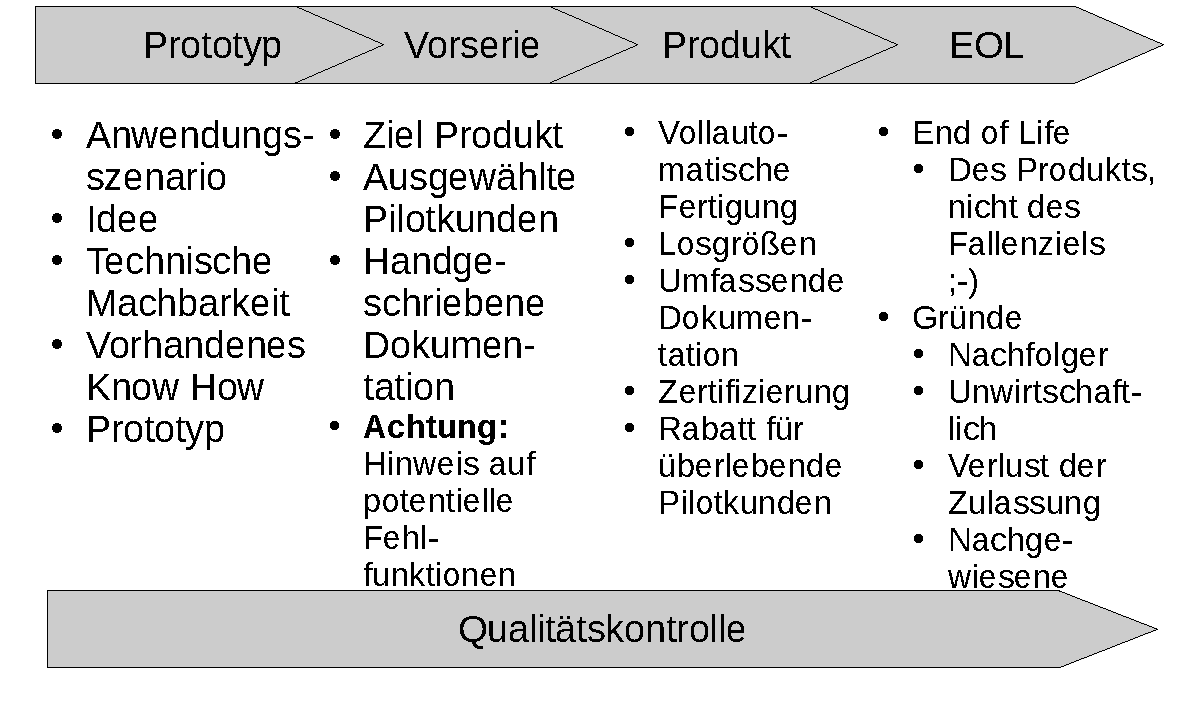
\includegraphics[width=.9\textwidth]{res/ablauf}
        \caption{Lebenszyklus eines Produkts von ACME Inc.}
        \label{fig:lifecycle}
    \end{figure}
    berücksichtigt werden.\marginpar{Fokus auf Ihren Aufgaben}
    Ziel ist dabei immer den Umsatz in einem Segment aus Tabelle~\ref{tab:umsatz}
    zu steigern.
    \begin{table}[htp]
        \centering
        \begin{tabular}{l|rrrrrrrrrr}
            Fallentyp/Jahre    & 56 & 57 & 58 & 59 & 60 & 61 & 62 & 63 & 64 & 65 \\\hline\hline
            Mechanische Fallen & 1  & 3  & 5  & 8  & 8  &  8 &  5 &  5 & 10 & 7 \\
            Raketenfallen      & -  & -  & -  & 2  & 3  &  6 &  7 &  9 &  3 & 2 \\
            Bogen              & 2  & 3  & 2  & 2  & 3  &  4 &  3 &  2 &  2 & 3 \\
        \end{tabular}
        \caption{Umsatz-Segmente von ACME Inc. von 1956--1965, in Tausend Dollar}
        \label{tab:umsatz}
    \end{table}
    Langfristig sollte dann aber meist auch die Funktionalität garantiert
    werden können.
    Im Praktikum \ldots


%% > weg damit
    \vskip\medskipamount % or other desired dimension
    \leaders\vrule width \textwidth\vskip0.4pt
    \vskip\medskipamount % ditto
    \nointerlineskip

    Bitte lesen Sie die Informationen zum Praxissemester~\cite{psmoodle}
    der Fakultät in Moodle.
    Sie halten sich an die Vorgaben im
    „Leitfaden zur Berichterstellung“~\cite{psberichtleitfaden},
    der auch in Moodle erhältlich ist.
    Für Hinweise zu \LaTeX~\cite{kopka,lamport,bibtexing,knuth} und zum
    Anfertigen einer Ausarbeitung~\cite{gockel,rechenberg} lesen Sie bitte
    auch das Thesis-Template in der
    Moodle Gruppe \texttt{PraxissemesterThesis}~\cite{psmoodle}.
    Ernsthaft, lesen Sie das Thesis-Template.
    Da stehen wirklich Hinweise zum Schreiben.
    Sie sollen dann durchaus viele Abbildungen und gegebenenfalls auch
    Tabellen in Ihren Text einbringen und nicht, wie hier im Template,
    nur Textwüsten.

    Die Vorstellung der Firma\marginpar{Vorstellung der Firma}
    braucht meist kein eigenes Kapitel und auf keinen Fall ein Logo.
    Sie machen selten eine Analyse der Firmenstruktur und die
    historische Entwicklung der Firma macht nur Seiten, aber hilft
    inhaltlich nicht.
    Also schreiben Sie in der Einleitung maximal nur einen Absatz
    zu der Firma und der Abteilung und konzentrieren sich dann auch
    die Inhalte.
    Wir schließen die Einleitung mit einer inhaltlichen Übersicht
    über die folgenden Kapitel.

    In Kapitel~\ref{ch:ppv} stellen wir die drei typischen Fallenprodukte
    vor sowie die passenden Prüfverfahren zur Verbesserung der
    mechanischen Genauigkeit und zur Reduktion der zeitlichen Verzögerung.
    In Kapitel~\ref{ch:sling} erläutern wir den Aufbau und das Messverfahren
    für die Abweichung von Schleudern beim Einsatz von schweren Gewichten
    über mehrere Tonnen.
    In Kapitel~\ref{ch:rocket} besprechen wir die erzielte Auslösereaktion
    durch Einsatz adäquater Sortierverfahren auf dem Mikrocontroller für die
    Raketensteuerung.
    Die Verbesserungen der Benutzbarkeit von Bögen unter Einsatz moderner Technik
    sammeln wir in Kapitel~\ref{chap:bow}.
    Abschließend fassen wir in Kapitel~\ref{chap:fazit} die im Praktikum
    erzielten mechanischen und zeitlichen Verbesserungen sowie die
    erhöhte Benutzbarkeit noch einmal zusammen.


    \chapter{Produkte und Prüfverfahren} \label{ch:ppv}

    Trotz Fokus auf den Anwendungsbereich Fallen wird ein weiter Bereich
    von technischer Infrastruktur im Produktangebot abgedeckt.
    Die eingesetzten Prüfverfahren testen meist eine mechanische
    und zeitliche Genauigkeit.

    \section{Schleudern, Raketen und Bögen} \label{sec:was}

    \blindtext[1]

    \section{Mechanische Genauigkeit} \label{sec:mec}

    \blindtext[1]

    \section{Zeitliche Abweichungen} \label{sec:time}

    \blindtext[1]

    \chapter{Genauigkeit von Schleudern} \label{ch:sling}

    Die Genauigkeit von Schleudern hängt von den beiden Faktoren
    Eins und Zwei ab und wird mit Drei oder Vier gemessen.
    Eins kombiniert X und Y, um qualitative Aussagen über den
    strukturellen Aufbau zu machen.
    Im Gegensatz dazu setzt sich Zwei aus A, B und C zusammen
    und erlaubt eine quantitative Festlegung.
    Das Verfahren Drei liefert mit wenig Aufwand einen ersten
    Anhaltspunkt, ob weitere detaillierte Messungen notwendig sind.
    Mit dem aufwendigen Verfahren Vier können wir dann Toleranzen
    auf $\pm 0.1\%$ Abweichung bestimmen.

    \section{Eins}

    \blindtext[1]

    \section{Zwei}

    \blindtext[1]

    \section{Drei}

    \blindtext[1]

    \chapter{Steuern von Raketentriebwerken} \label{ch:rocket}

    Raketentriebwerke werden hauptsächlich mechanisch gesteuert.
    Nur das Anstoßen von Zustandsübergängen Zwei wird elektronisch
    getriggert.
    Drei ist eine übliche Realisierung.

    \section{Eins}

    \blindtext[1]

    \section{Zwei}

    \blindtext[1]

    \section{Drei}

    \blindtext[1]

    \chapter{Benutzbarkeit von Bögen} \label{chap:bow}

    Text\ldots

    \section{Eins}

    \blindtext[1]

    \section{Zwei}

    \blindtext[1]

    \section{Drei}

    \blindtext[1]


    \chapter{Fazit} \label{chap:fazit}

    \blindtext[1]


    \newpage

% Listen wenn überhaupt ans Ende und nicht an den Anfang.
% Meist ist das aber unnötig.
    \listoffigures % Liste der Abbildungen
%\begingroup % aahh nicht noch ein pagebreak
%\let\clearpage\relax %
    \listoftables % Liste der Tabellen
%\endgroup

% Glossar kommt auch ans Ende
%\glsaddall % das fügt alle Glossar-Einträge ein
%\printglossaries % nicht vergessen "makeglossaries praksem" aufzurufen
%\gls{Computer}
%\newpage

    \addcontentsline{toc}{chapter}{Literaturverzeichnis}
    \bibliographystyle{plain} % Literaturverzeichnis
    \bibliography{praksem}
% \bibliography{praksem,online} # wenn man zwei Dateien hätte

% Das wäre die Alternative mit geteilten Quellen (preamble muss auch
% angepasst werden) und die Literatur muss in die Datei praksem.bib
% und die Online-Quellen müssen in die Datei online.bib.
%\begin{btSect}{praksem} % mit bibtopic Quellen trennen
%\section*{Literaturverzeichnis}
%\addcontentsline{toc}{chapter}{Literaturverzeichnis}
%\btPrintCited
%\end{btSect}
%\begin{btSect}{online}
%\section*{Online-Quellen}
%\addcontentsline{toc}{chapter}{Online-Quellen}
%\btPrintCited
%\end{btSect}
% dann ab und zu "bibtex praksem1" und "bibtex praksem2" aufrufen

\end{document}
;;; Local Variables:
;;; ispell-local-dictionary: "de_DE-neu"
;;; End:
